%请认真填写有关内容,勿删相关信息
%由于学校很多内容有特殊要求,请掌握规律后进行相应的编写。
%由于本人有限,所以需要填的东西较多,且所见即所得的情况比较多,请原谅,欢迎各位道友指正。
%也欢迎农大的老师同学进行相应的改正。
%非常感谢帮助过我的人,也欢迎大家继续修改,让模板越来越简单,让LaTeX写作称为一种习惯
%需要注意的是再填写完chapter、section、subsection之后请相应加入echapter、esection、esubsection
%如果题目2行仍然过长请在cls里修改dlmu的长度,我在相关地方注释了



\documentclass{SDAUthesis}
\graphicspath{{figures/}}
\begin{document}
\author{黄泽盛}									%作者
\authorEn{Huang Ze sheng}				%作者的中文
\advisor{郭鹏}								%指导老师
\advisors{郭鹏(副教授)}					%指导老师带有职称
\advisorEn{Guo peng}						%指导老师的英文
\college{信息科学与工程学院}				%学院
\serialnumber{20177740}																	%学号				
\grade{2021届}							%届数	
\major{遥感17-2}							%专业班级
\submityear{二 \ 一 \ }%提交年份二〇二〇就填二〇,斜号控制距离,请勿乱删
\submitmonth{六}  					%提交的月份
\submitdate{五}	
\titleZh{山东农业大学信息学院学士学位\LaTeX 模板  }				%第二页的中文标题
\titleEn{\LaTeX  \ template of bachelor's degree from school of information, Shandong Agricultural University}     %第二页的英文标题
\majorEn{Remote Sensing}											%专业英文
\majorZh{遥感科学与技术}							%专业中文
\titlefirst{山东农业大学信息学院学士学位}    %标题第一行
\titlesecond{ \LaTeX 模板(非官方)}	%标题第二行

\majortotal{2017级遥感科学与技术}		%年级+专业

%完成封面页

%请勿删除,对于生成封面页非常重要
\maketitle
% !TEX encoding = UTF-8
%定义英文目录使用请勿删
\makeatletter
\newcommand\engcontentsname{Contents}
\newcommand\tableofengcontents{%
	\if@twocolumn
	\@restonecoltrue\onecolumn
	\else
	\@restonecolfalse
	\fi
	\chapter*{\engcontentsname
		\@mkboth{%
			\MakeUppercase\engcontentsname}{\MakeUppercase\engcontentsname}}%
	\@starttoc{toe}% !!!!Define a new contents!!!!
	\if@restonecol\twocolumn\fi
	
}
\newcommand\addengcontents[2]{%
	\addcontentsline{toe}{#1}{\protect\numberline{\csname the#1\endcsname}#2}}
\makeatother

\newcommand\echapter[1]{\addengcontents{chapter}{#1}}
\newcommand\esection[1]{\addengcontents{section}{#1}}
\newcommand\esubsection[1]{\addengcontents{subsection}{#1}}

\tableofcontents
\tableofengcontents\thispagestyle{empty}

%摘要页,前往abstract进行填写相关内容,请一边编辑一边观看效果
% !TEX encoding = UTF-8
%摘要部分
\Chabstract{本模板按照山东农业大学信息学院毕业设计(参考版)设计,由于\LaTeX 和Word存在一些差别,所以无法做到百分之百的一样,但是,本人在编写过程中已经尽量使得格式符合学院的要求,由于不清楚是否符合学院的要求,需要老师鉴定或者认可之后才能使用进行论文的撰写。需要注意的是,由于模板中需要有华文行楷和方正小标宋简体的字体,如果用户没有该字体需要进行下载,同时学院要求要有word,不推荐\LaTeX 转word,容易识别错误或者其他致命的错误。}
\Chkeyword{拉泰赫;模板;毕业设计}
\Enabstract{This template is designed according to the graduation design (Reference Version) of School of information of Shandong Agricultural University There are some differences with word, so it can't be 100\% the same. However, in the process of writing, I have tried to make the format meet the requirements of the college. Because I don't know whether it meets the requirements of the college, I need the teacher's appraisal or approval before I can write the thesis. It should be noted that because the template needs to have the font of Chinese line regular script and founder small mark song simplified Chinese, if the user does not have the font, they need to download it. At the same time, the college requires word, and it is not recommended to convert the word from latex, which is easy to identify.}	%英文摘要
\Enkeyword{\LaTeX;Template;Graduation project}				%首字母大写
%摘要页面
\totalabstract


%中文的摘要



\mainmatter

%chapter1
% !TEX encoding = UTF-8
%勿必别忘了添加echapter

%第一章
\chapter{数学公式和定理类环境}
\echapter{Mathematical formula and Theorem environment }

\section{定理环境}
\esection{Theorem environment }											

%推论
\begin{corollary}\label{cor1}
推论测试
\end{corollary}


%定理
\begin{theorem}\label{thm1}
定理测试
\end{theorem}

%定义测试
\begin{definition}\label{def1}
定义测试
\end{definition}

%公理
\begin{axiom}\label{axi1}
公理测试
\end{axiom}

%接下来很多就都不测试了,后面表格有已经定义了的定理等的环境总结。


\section{数学公式}
\esection{mathematical formulas}

\par 数学公式是使用许多人使用\LaTeX 的一大原因,\LaTeX 排版出来的公式美观,格式统一,不需要过多的操心。编号等基本的设置已经设置完成。


\begin{equation}
	NDVI  =  \frac{NIR-Red}{NIR+Red}	
\end{equation}


\begin{align} 
	 x   &   =  t  + \cos t + 1 \\
	 y   &  = 2 \sin t
\end{align}


\[ \begin{pmatrix}
        1    &         2\\ 
        2    &         3  
\end{pmatrix}			\label{matrix}  
\]







%chapter2										%如是下去自行变化
% !TEX encoding = UTF-8
\chapter{图片}
\echapter{pictures}


由于图片和表格处于浮动题环境内,初始看到请不要惊讶,后期完成后会自动调整,尽量不要用强制位置,容易造成页面的不协调,如果真的需要强制使用,可以使用captionof进行标号,但是非常不建议这样使用

\begin{figure}[!htbp]
	  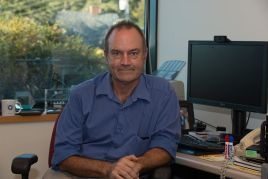
\includegraphics[width=10.5cm]{canny.jpg}
	  \centering
	  \caption{Canny边缘提取算法创始人}
	  \label{canny}
\end{figure}



\begin{tcode}
	\begin{figure}[!htbp]
		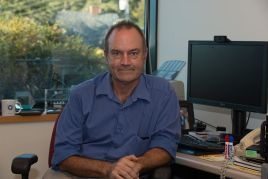
\includegraphics[scale=0.5]{canny.jpg}
		\centering
		\caption{Canny边缘提取算法创始人}
		\label{canny}
	\end{figure}
\end{tcode}
如果想使用非浮动题环境或者软强制定位图片,在附加参数选项中加入[!htbp]或者使用captionof命令,例如:

{
	\centering
	
\includegraphics[scale=0.5]{SDAU.jpg}
	\captionof{figure}{山东农业大学校徽}
	\label{xiaohui}
}

\begin{tcode}
	{
		\centering
		
\includegraphics[scale=0.5]{SDAU.jpg}
		\captionof{figure}{山东农业大学校徽}
		\label{xiaohui}
	}
\end{tcode}
更多关于插图的技巧请自行阅读我在文件夹中留下的插图手册,或者自行观看工作室的直播。直播的链接为:
\href{https://www.bilibili.com/video/BV1nv41117q9}{https://www.bilibili.com/video/BV1nv41117q9}.
如果需要绘制矢量图,请自行阅读tikz帮助文档,或者在小屋内下载相关作者翻译的文档,或者使用ppt、visio等软件绘制


%tikz的工作示例
\begin{figure}
	\centering
	\begin{tikzpicture}
\node (ciji)  [] at (-0.5,0) {刺激};
\node (ganshouqi)[draw,minimum height = 0.8cm,thick] at (1.5,0)  {感受器};
\node (shenjing)    [draw,minimum height = 0.8cm,thick]  at (4,0) {神经网络};
\node (xiaoying)   [draw,minimum height = 0.8cm,thick] at (6.5,0) {效应器};
\node (xiangying) [minimum height = 0.8cm,thick] at (8.5,0) {响应};
		\draw [-stealth]  (ciji.east) -- (ganshouqi.west);
\draw [-stealth] ($(ganshouqi.east) + (0, 2mm)$) -- ($(shenjing.west) + (0,
2mm)$);
\draw [-stealth] ($(shenjing.west) + (0, -2mm)$) -- ($(ganshouqi.east) + (0,
-2mm)$);
\draw [-stealth] ($ (shenjing.east) + (0,2mm) $)  -- ($(xiaoying.west) + (0,2mm) $);
\draw [-stealth] ($ (xiaoying.west) + (0,-2mm) $)  -- ($(shenjing.east) + (0,-2mm) $);
\draw [-stealth] (xiaoying.east) -- (xiangying.west); 
	\end{tikzpicture}
   \caption{神经网络}
\end{figure}

%tikz的代码
\begin{tcode}
\begin{figure}
	\centering
	\begin{tikzpicture}
	\node (ciji)  [] at (-0.5,0) {刺激};
	\node (ganshouqi)[draw,minimum height = 0.8cm,thick] at (1.5,0)  {感受器};
	\node (shenjing)    [draw,minimum height = 0.8cm,thick]  at (4,0) {神经网络};
	\node (xiaoying)   [draw,minimum height = 0.8cm,thick] at (6.5,0) {效应器};
	\node (xiangying) [minimum height = 0.8cm,thick] at (8.5,0) {响应};
	\draw [-stealth]  (ciji.east) -- (ganshouqi.west);
	\draw [-stealth] ($(ganshouqi.east) + (0, 2mm)$) -- ($(shenjing.west) + (0,
	2mm)$);
	\draw [-stealth] ($(shenjing.west) + (0, -2mm)$) -- ($(ganshouqi.east) + (0,
	-2mm)$);
	\draw [-stealth] ($ (shenjing.east) + (0,2mm) $)  -- ($(xiaoying.west) + (0,2mm) $);
	\draw [-stealth] ($ (xiaoying.west) + (0,-2mm) $)  -- ($(shenjing.east) + (0,-2mm) $);
	\draw [-stealth] (xiaoying.east) -- (xiangying.west); 
	\end{tikzpicture}
   \caption{神经网络}
\end{figure}

\end{tcode}


%chapter3
% !TEX encoding = UTF-8
\chapter{表格}
\echapter{chart}

由于格式要求表格字体内为5号字,所以需要自己在table和tabular环境前加上 \verb|\zihao{5}| \\的代码,可以参照工作示例。
表格可以使用浮动体或者非浮动体的方式,建议没有强迫症的同学还是使用浮动体的环境,如果有强迫症的同学也还是稍微改一改,如果非要选择非浮动题环境,那么参考下面的工作示例。

\begin{tcode}
%浮动题环境示例
\begin{table}
	\zihao{5}
	\centering
	\caption{已经定义了的定理}
	\begin{tabular}{|c|c|}
		\hline               
		定义      &   definition  \\   \hline 
		定理      &   theorem    \\   \hline
		公理      &   axiom		\\   \hline
		引理		&	lemma		\\   \hline
		命题	   &	proposition \\  \hline
		注		  &	  remark		\\  \hline
		解		  &	  solution   \\ \hline
		证明		&	proofname  \\ \hline
		
	\end{tabular}
\end{table}
\end{tcode}

%浮动题环境示例
\begin{table}
	\zihao{5}
	\centering
	\caption{已经定义了的定理}
	\begin{tabular}{|c|c|}
		\hline               
		定义      &   definition  \\   \hline 
		定理      &   theorem    \\   \hline
		公理      &   axiom		\\   \hline
		引理		&	lemma		\\   \hline
		命题	   &	proposition \\  \hline
		注		  &	  remark		\\  \hline
		解		  &	  solution   \\ \hline
		证明		&	proofname  \\ \hline
	\end{tabular}
\end{table}


%非浮动题工作代码示例。
%由于captionof针对非浮动体,所以它距离所需要的表或者线的垂直距离变成了0,由于book、article等类的间距为10pt所以需要加入vspace=10pt
\begin{tcode}
	{%非浮动题工作代码示例。
		\zihao{5}	
		\centering
		\captionof{table}{已经定义了的定理}
		\vspace{10pt}				
		\begin{tabular}{|c|c|}
			\hline               
			定义      &   definition  \\   \hline 
			定理      &   theorem    \\   \hline
			公理      &   axiom		\\   \hline
			引理		&	lemma		\\   \hline
			命题	   &	proposition \\  \hline
			注		  &	  remark		\\  \hline
			解		  &	  solution   \\ \hline
			证明		&	proofname  \\ \hline
				\end{tabular}
	}
\end{tcode}

%非浮动题环境
	{
	\zihao{5}
	\centering
	\captionof{table}{已经定义了的定理}
	\vspace{10pt}
	\begin{tabular}{|c|c|}
		\hline               
		定义      &   definition  \\   \hline 
		定理      &   theorem    \\   \hline
		公理      &   axiom		\\   \hline
		引理		&	lemma		\\   \hline
		命题	   &	proposition \\  \hline
		注		  &	  remark		\\  \hline
		解		  &	  solution   \\ \hline
		证明		&	proofname  \\ \hline
	\end{tabular}

}




%chapter4
% !TEX encoding = UTF-8
%请勿忘记添加echapter
\chapter{如何添加参考文献}
\echapter{How to add references}

\par 其实刘梦良老师是建议使用bibitem的方式的,但是由于本人还是习惯使用bibtex,请使用者自行利用jabref或者Google  Scholar 的镜像添加bibtex里面的内容,再使用cite进行引用,本人就不过多的赘述了\cite{朱建章2016遥感大数据研究现状与发展趋势},使用的是gbt7714的宏包,基本已经能够满足gbt7714的格式要求\cite{lary2016machine}。



%chapter4
% !TEX encoding = UTF-8
%请勿忘记添加echapter
\chapter{注意事项}
\echapter{notice}

\begin{enumerate}
	\item 本模板为非官方模板,需要学院认可方可使用。
	\item 由于word和\LaTeX 固有的差别,不可能$100$\% 复现word效果。
	\item 创建了一个山东农业大学\LaTeX 交流群,群号为835684647,欢迎感兴趣的老师同学加入。
	\item 如果有什么多余需要和错误改正,请加入交流群联系作者。
	\item 祝大家能够快乐的使用\LaTeX , Happy \LaTeX ing!
\end{enumerate}


%bib文件,请利用jabref或者谷歌学术镜像导出bibtex后加入reference
\addcontentsline{toe}{chapter}{Reference}
{\zihao{-4}
\bibliography{reference}
}
%参考文献放入中文目录
\addcontentsline{toc}{chapter}{参考文献} 

%致谢的文件,前往相应文件进行编辑
% !TEX encoding = UTF-8
\Thanks
\addcontentsline{toe}{chapter}{Acknowledgement}
非常感谢各位朋友的帮助,让我在几天时间内完成了本学位模板的撰写,虽然还有很多不完善的地方,但是还希望大家多多包涵,本人能力还有限,也希望在大家提完问题之后我能够有机会或者能力去修改补充内容,也希望越来越多的高校能够拥有\LaTeX 模板,并且将其推广开来,让格式不再成为写作的拦路虎,希望后续农大有人能够完善这个模板。
在此,在这里感谢ChinaTeX的版主,能够帮我纠正错误,同时也感谢湖南师范大学\LaTeX 模板的撰写人,能够回答我的一些问题,也感谢数学系的刘梦良老师,在大家的共同帮助下我能够完成这个模板的撰写。

%附录的文件,前往相应文件进行编辑
% !TEX encoding = UTF-8
%附录内容,自行修改
\Appendix																   %勿删
\addcontentsline{toe}{chapter}{Appendix}             %加入英文的目录,请勿删去.

\begin{lstlisting}[language=MATLAB]
function [] = m1_callback(source,evendata)
	handles = guidata(source);
	[filename,path] = uigetfile({'*.';'*.jpg';'*.png';'*.jpeg';'*.bmp';;},'选择图片');
	try  isa(filename,'numeric');                       
		truename = [ path,filename ];              %拼接真正的路径名
		im = imread(truename);                        %显示图片
		subplot(2,3,1);                         
		imshow(im);
		chicun = size(im);
	switch numel(chicun)
		case 2
		im1 = im;
		case 3
		im1 = rgb2gray(im);
	end
		im1 = double(im1);                                 %读入的是uint8类型,要转double才能计算
		handles.im1 = im1;
		guidata(source,handles);
		title('原始图像','fontsize',20);
		catch
	warn = errordlg('你取消了选择,请勾选文件','File Error');
	end
end
\end{lstlisting}

\begin{lstlisting}[language = python]
##!/usr/bin/python## -*- 
coding: UTF-8 -*-
#flag判断标志 number_sum为总和
	flag = True
	number_sum = 0
	while flag == True:   
	number_a = input('Please Enter a number: ')    
	number_b = input('Please Enter another number: ')  
	try:          
	a = int(number_a)  
	b = int(number_b)   
	except ValueError:        
	print('You have Entered wrong number')    
	else:        
	number_sum = a + b     
	print('The sum of two numbers: ' + str(number_sum))
	flag = False
\end{lstlisting}


%附件的文件,前往相应文件进行编辑
% !TEX encoding = UTF-8
\fujian 















\end{document}